\section{A fixed rank-five bundle with separated spectral scales}\label{sec:example}

We give a geometric example in which the stable region has three
independent polarization parameters. Its full finite model has six
complex modes, and one can tend to zero at an arbitrary positive
rate relative to the other five.

Let $X=(\PP^1)^4$. Write $\omega_\ell$ for the pullbacks of
Fubini--Study forms normalized by $\int_{\PP^1}\omega_\ell=1$,
and put $\omega_h=\sum_{\ell=1}^4h_\ell\omega_\ell$, with
$h_\ell>0$. Consider
\begin{equation}\label{eq:linebundles}
F_0=\mathcal O_X,\qquad F_j=\mathcal O_X(2e_j-2e_4)\quad(1\le j\le3),
\end{equation}
where $e_\ell$ denotes degree one on the $\ell$-th factor, and
an extension
\begin{equation}\label{eq:star-extension}
0\longrightarrow\mathcal O_X\otimes\C^2\longrightarrow E
\longrightarrow F_1\oplus F_2\oplus F_3\longrightarrow0.
\end{equation}
All four stable types are line bundles. They are distinct and have
degree zero at $h=(1,1,1,1)$. Product invariant Hermitian metrics are
HE for every product polarization. The normalization
\eqref{eq:degree} gives
\begin{equation}\label{eq:linecurvature}
V_h=h_1h_2h_3h_4,\qquad\kappa_0=0,\qquad
\kappa_j=4\pi(h_j^{-1}-h_4^{-1}),\qquad
\kappa_E=\tfrac15\sum_{j=1}^3\kappa_j.
\end{equation}
Indeed $iF_{F_j}=4\pi(\omega_j-\omega_4)$ and
$\Lambda_{\omega_h}\omega_\ell=h_\ell^{-1}$.

The Künneth formula and line-bundle cohomology on $\PP^1$ give
\begin{equation}\label{eq:extstar}
\Ext^1(F_j,F_0)=
H^1(\PP^1,\mathcal O(-2))\otimes H^0(\PP^1,\mathcal O(2))
\cong\C^3.
\end{equation}
The nonconstant factors are $j$ and $4$; the others contribute
$H^0(\mathcal O)=\C$. Fix cohomology bases orthonormal at the
reference polarization in the volume-normalized inner product.
For every $h$, the current harmonic Gram matrix is $c_j(h)I_3$
with $c_j(h)>0$ smooth. To see this, all the chosen metrics and
forms are invariant under $\mathrm{SU}(2)^4$. The only nontrivial
action on \eqref{eq:extstar} is the irreducible three-dimensional
representation on the fourth-factor degree-two sections.
Schur's lemma makes the invariant harmonic inner product a scalar
multiple of the reference one. The cohomology coefficients below
remain fixed as the harmonic representatives vary.

For small real $a=(a_1,a_2,a_3)$ let $A=a_1+a_2+a_3$ and choose
the actual polarization chart
\begin{equation}\label{eq:chart}
h_4=1,\qquad
h_j=\left(1+\frac{A/2+a_j}{4\pi}\right)^{-1}\quad(1\le j\le3).
\end{equation}
It is defined for all sufficiently small signed $a$ and has
positive coefficients. Substitution into \eqref{eq:linecurvature}
gives
\begin{equation}\label{eq:demands}
\kappa_E=A/2,\qquad\kappa_j-\kappa_E=a_j,\qquad
b_0=A/2,\qquad b_j=-a_j,\qquad\sigma=A.
\end{equation}
The target moment is $(A/2)I_2$, so its trace is $A$. Thus the
three finite demands are independent geometric parameters.

\subsection{The extension and its complete endomorphism algebra}
Define the fixed extension class by the following matrices, whose
three columns multiply the basis elements in \eqref{eq:extstar}:
\begin{equation}\label{eq:Zstar}
\begin{split}
Z_1^0&=\begin{pmatrix}\sqrt{3/2}&0&0\\0&1/\sqrt2&0\end{pmatrix},\qquad
Z_2^0=\begin{pmatrix}1&0&0\\1/2&\sqrt3/2&0\end{pmatrix},\\
Z_3^0&=\begin{pmatrix}1/\sqrt2&0&0\\-1/\sqrt2&1&0\end{pmatrix}.
\end{split}
\end{equation}
An extension of locally free sheaves by locally free sheaves is
locally free. These classes therefore define one fixed rank-five
holomorphic bundle, rather than merely a finite representation.
The covariances $B_j=Z_j^0(Z_j^0)^*$ are
\begin{equation}\label{eq:Bstar}
B_1=\begin{pmatrix}3/2&0\\0&1/2\end{pmatrix},\quad
B_2=\begin{pmatrix}1&1/2\\1/2&1\end{pmatrix},\quad
B_3=\begin{pmatrix}1/2&-1/2\\-1/2&3/2\end{pmatrix}.
\end{equation}
They have determinants $3/4,3/4,1/2$, respectively, and
\begin{equation}\label{eq:noncommute}
B_1+B_2+B_3=3I_2,\qquad
[B_1,B_2]=\begin{pmatrix}0&1/2\\-1/2&0\end{pmatrix}\ne0.
\end{equation}
In particular the interactions are not simultaneously diagonal.

If $XZ_j^0=Z_j^0x_j$ for $X\in M_2(\C)$ and scalar $x_j$,
full row rank of each $Z_j^0$ implies $X=x_jI_2$.
All $x_j$ coincide. Lemma~\ref{lem:algebra} proves that $E$ is
simple. The full trace-free complex space is
\begin{equation}\label{eq:starspace}
\HH=\{(X,x_1,x_2,x_3):\tr X+x_1+x_2+x_3=0\},\qquad
\|(X,x)\|^2=\|X\|_F^2+\sum_j|x_j|^2.
\end{equation}
It has dimension six. The multiplicity two of the target is
already included in its matrix trace; it is not an additional
factor rank.

\begin{proposition}\label{prop:starbalance}
The local stable region of the fixed bundle \eqref{eq:star-extension}
in the chart \eqref{eq:chart} is exactly $a_1,a_2,a_3>0$.
For these parameters its balanced covariances are
\begin{equation}\label{eq:targetbalance}
C_j=a_j\frac{TB_jT}{\tr(TB_jT)},\qquad
\sum_{j=1}^3C_j=\frac A2I_2,
\end{equation}
where $T$ is positive Hermitian and $\det T=1$.
The target shape $T$ is unique, uniformly bounded together with
its inverse, and smooth in the normalized weights $w_j=a_j/A$
on the entire closed simplex.
\end{proposition}

\begin{proof}
If a subrepresentation contains any source, its target contains
the span of that source's three images, which is all of $\C^2$.
The proper nonzero subrepresentations therefore have either a
target line and no sources, or the full target with a proper
subset $S$ of sources. Their demands are $A/2$ and
$\sum_{j\notin S}a_j$, respectively. They are all positive
when $a_j>0$. Conversely, taking the full target and every
source except $j$ gives demand $a_j$, so finite stability
requires all three to be positive. Theorem~\ref{thm:main}
identifies this with the actual local stable region.

The scalar harmonic Gram factor $c_j(h)$ can be absorbed into
the positive gauge at source $j$. After a target gauge $T$,
choose its source multiplier to have square
$c_j(h)\tr(TB_jT)/a_j$. This produces \eqref{eq:targetbalance}
in the same extension orbit. A common scalar on all blocks
normalizes the entire bundle determinant; $\det T=1$ fixes only
the target shape.

To prove existence and uniformity directly, put $H=T^2$ and
minimize
\begin{equation}\label{eq:targetpotential}
f_w(H)=\sum_jw_j\log\tr(HB_j),\qquad H=H^*>0,\quad\det H=1.
\end{equation}
All $B_j$ are positive definite. With $c=1-1/\sqrt2>0$,
one has $B_j\ge cI$ and $f_w(I)=\log2$. Therefore
\[
f_w(H)\ge\log(c\tr H),\qquad
\tr H\le\frac2c=4+2\sqrt2
\quad\text{at a minimizer}.
\]
This is a uniform coercivity bound for all weights in the
closed simplex. The determinant condition bounds both
eigenvalues above and away from zero on the indicated sublevel
set, proving existence and compactness of the minimizers.

For a determinant-one geodesic
$H(t)=H_0^{1/2}e^{tY}H_0^{1/2}$ with $Y=Y^*$ and $\tr Y=0$,
each summand of \eqref{eq:targetpotential} is
$\log\sum_\ell q_{j\ell}e^{ty_\ell}$ in an eigenbasis for $Y$.
Every $q_{j\ell}$ is strictly positive, because $B_j>0$.
The second derivative is the variance of the $y_\ell$ under
positive normalized weights. It is strictly positive when
$Y\ne0$. A convex combination of these variances remains
positive even if some $w_j=0$. Hence $f_w$ is strictly geodesically
convex and the minimizer is unique.

At $H=T^2$ its first variation in direction $TYT$ is
\[
\tr\left(Y\sum_jw_j\frac{TB_jT}{\tr(TB_jT)}\right).
\]
It vanishes for every trace-free Hermitian $Y$ exactly when the
matrix in parentheses is $I_2/2$, proving
\eqref{eq:targetbalance}. On the compact family of minimizers
the Hessian has a uniform positive lower bound on unit tangent
vectors. The finite-dimensional implicit-function theorem gives
a smooth extension near each point of the closed simplex in its
affine weight hyperplane. Uniqueness patches these extensions.
This proves the asserted smoothness, including at corners.
\end{proof}

At a boundary weight the corresponding limiting arrow disappears.
The source gauge relating it to the original nonzero class is no
longer invertible there. Boundedness of $T$ is not boundedness of
the full metric, and the proposition asserts no HE metric on the
original boundary bundle.

\subsection{Six finite modes}
For the covariances \eqref{eq:targetbalance}, the finite form is
\begin{equation}\label{eq:starform}
\mathcal Q(X,x)=\sum_{j=1}^3
\tr\bigl((X-x_jI)C_j(X-x_jI)^*\bigr)
\quad\text{on \eqref{eq:starspace}}.
\end{equation}
At $a_1=a_2=a_3=2t$ one has $T=I$ and $C_j=tB_j$.

\begin{proposition}\label{prop:sixmodes}
At these equal demands the six finite eigenvalues, divided by $t$,
are
\begin{equation}\label{eq:sixmodes}
3,\quad5,\quad\frac{5-\sqrt7}{2},\quad\frac{5+\sqrt7}{2},\quad
\frac{5-\sqrt3}{2},\quad\frac{5+\sqrt3}{2}.
\end{equation}
The scalar-target compression instead has only three positive
eigenvalues, $2t,2t,5t$.
\end{proposition}

\begin{proof}
It suffices to take $t=1$. In $M_2(\C)$ use the orthonormal basis
\[
I_2/\sqrt2,\qquad\sigma_z/\sqrt2,\qquad
\sigma_x/\sqrt2,\qquad\sigma_y/\sqrt2,
\]
where the last three are the Pauli matrices. Their complex span
is the full matrix algebra. On the complete seven-dimensional
space before removing the identity, \eqref{eq:starform} has matrix
\begin{equation}\label{eq:staroperator}
L=\begin{pmatrix}3I_4&-K\\-K^*&2I_3\end{pmatrix},\qquad
K=\begin{pmatrix}
\sqrt2&\sqrt2&\sqrt2\\
1/\sqrt2&0&-1/\sqrt2\\
0&1/\sqrt2&-1/\sqrt2\\
0&0&0
\end{pmatrix}.
\end{equation}
The eigenvalues of $K^*K$ are $6,3/2,1/2$.
Each squared singular value $s^2$ gives the quadratic factor
$(\lambda-3)(\lambda-2)-s^2$, and the remaining target
direction has eigenvalue $3$. Thus
\[
\det(\lambda I_7-L)=\lambda(\lambda-5)(\lambda-3)
(\lambda^2-5\lambda+9/2)(\lambda^2-5\lambda+11/2).
\]
The zero is exactly the scalar identity. Its orthogonal complement
is \eqref{eq:starspace}, which gives \eqref{eq:sixmodes}.
Restricting the target to its scalar part replaces $K$ by its
first row and gives $\lambda(\lambda-5)(\lambda-2)^2$.
\end{proof}

\subsection{Arbitrary separation on genuine polarizations}
Set $a=(t\delta,t,t)$, with $t,\delta>0$. The target solution
depends only on $w=(\delta,1,1)/(2+\delta)$, so the form
$\mathcal Q/t$ is smooth in $\delta$ down to zero.

\begin{theorem}\label{thm:star-scales}
There are $t_0,\delta_0,c,C,\gamma>0$ such that, for independently
chosen $0<t<t_0$ and $0<\delta<\delta_0$, the HE spectrum of the
fixed bundle \eqref{eq:star-extension} at \eqref{eq:chart} satisfies
\begin{equation}\label{eq:staractual}
\lambda_1=\frac54t\delta\bigl(1+O(\delta)+O(t)\bigr),\qquad
ct\le\lambda_j\le Ct\ (2\le j\le6),\qquad
\lambda_7\ge\gamma.
\end{equation}
All constants are independent of the ratio between $\delta$ and $t$.
\end{theorem}

\begin{proof}
At $\delta=0$ the target and sources $2,3$ form a simple
representation, since each of these sources has full image span.
The absent first source adds one centralizer direction. On
\eqref{eq:starspace} the kernel is therefore exactly the line
\begin{equation}\label{eq:weakkernel}
(X,x_1,x_2,x_3)=(\alpha I_2,-4\alpha,\alpha,\alpha).
\end{equation}
Its squared norm is $20|\alpha|^2$, and the remaining five
eigenvalues of $\mathcal Q/t$ are positive. On this fixed vector
the strong-source terms vanish for every target shape. Since
$\tr C_1=t\delta$, the weak-source term is exactly
$25t\delta|\alpha|^2$. Smooth perturbation of the simple zero
eigenvalue gives
\begin{equation}\label{eq:weakfinite}
\nu_1=\frac54t\delta\bigl(1+O(\delta)\bigr),\qquad
ct\le\nu_j\le Ct\quad(2\le j\le6).
\end{equation}
The derivative $5/4$ is the ratio $25/20$ of energy derivative
to mass. The finite form scales exactly with $t$, so these
constants are uniform in $t>0$.

All $a_j$ are positive, and
$\sigma=t(2+\delta)$. Theorem~\ref{thm:main} applies with
relative error $O(t)$ and a fixed complementary gap. Combining
it with \eqref{eq:weakfinite} proves \eqref{eq:staractual}.
\end{proof}

For every fixed $p>0$, the choice $\delta=t^p$ yields a small
eigenvalue of order $t^{p+1}$ while the other five have order $t$.
The choice $\delta=e^{-1/t}$ gives a faster separation. Both are
paths of actual Kähler polarizations of the same fixed bundle.

\begin{figure}[htbp]
\centering
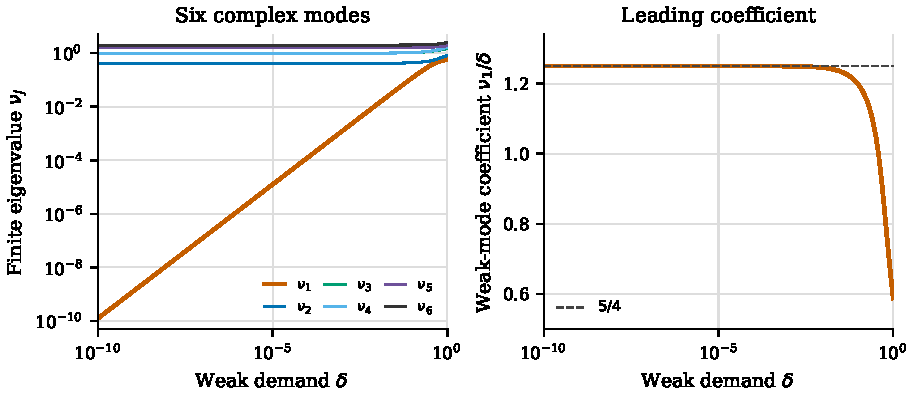
\includegraphics[width=\textwidth]{figures/output/weak_modes.pdf}
\caption{Finite commutator eigenvalues for demands $(\delta,1,1)$
(equivalently $t=1$ in the homogeneous finite model).
The first mode tends to zero while the other five stay positive;
the second panel displays its coefficient tending to $5/4$.
These are numerical evaluations of \eqref{eq:starform}, not
computed eigenvalues of the HE differential operator. Theorem~\ref{thm:star-scales}
supplies the relative comparison for small geometric $t$.}
\label{fig:weakmodes}
\end{figure}
